\documentclass[tikz]{standalone}
\usepackage{pgfplots}
\pgfplotsset{compat=1.15}
\usepackage{mathrsfs}
\usetikzlibrary{arrows,calc}
\usepackage{tkz-euclide}

\pagestyle{empty}

\definecolor{AngleClr}{rgb}{0,0.39215686274509803,0}
\definecolor{ShapeClr}{rgb}{0.6,0.2,0}
\definecolor{BlueClr}{RGB}{13,93,184}

\begin{document}

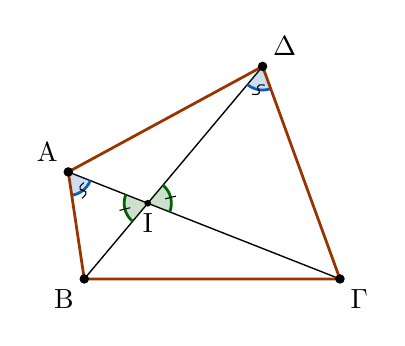
\begin{tikzpicture}[scale=.75]
\tkzSetUpLine[line width=1pt,color=black]
\tkzSetUpPoint[fill=black]

\tkzDefPoints{0/0/O}

\tkzDefPoint(167:2.5){A}
\tkzDefPoint(-150:2.5){B}
\tkzDefPoint(-30:2.5){C}
\tkzDefPoint(70:2.5){D}

\tkzInterLL(A,C)(B,D)\tkzGetPoint{I}

\tkzFillPolygon[fill=white](A,B,C,D)
\tkzDrawSegments[line width=0.5pt,color=black](A,C B,D)

\tkzFillAngles[fill=AngleClr,size=.4,fill opacity=0.2](C,I,D A,I,B)
\tkzMarkAngles[line width=1pt,size=.4,color=AngleClr,mark=|,mksize=2](C,I,D A,I,B)

\tkzFillAngles[fill=BlueClr,size=.4,fill opacity=0.2](B,A,I B,D,C)
\tkzMarkAngles[line width=1pt,size=.4,color=BlueClr,mark=s,mksize=2](B,A,I B,D,C)

\tkzDrawPolygon[color=ShapeClr](A,B,C,D)

\tkzDrawPoints[size=3](A,B,C,D)
\tkzDrawPoints[size=2](I)
\tkzLabelPoint[above left](A){$\rm A$}
\tkzLabelPoint[below left](B){$\rm B$}
\tkzLabelPoint[below right](C){$\rm \Gamma$}
\tkzLabelPoint[above right](D){$\rm \Delta$}
\tkzLabelPoint[below](I){$\rm I$}

\end{tikzpicture}
\end{document}
